\documentclass{article}
\usepackage{graphicx,fancyhdr,amsmath,amssymb,amsthm,subfig,url,hyperref}
\usepackage[margin=1in]{geometry}
\usepackage{xltxtra}
\usepackage{xgreek}
\usepackage{amsfonts}
\usepackage{amssymb}
\usepackage{amsmath}
\usepackage{graphicx}
\usepackage{listings}
\usepackage{framed}
\usepackage{minted}
\usepackage{caption}
\usepackage{ subfig}
%\setmainfont[Mapping=tex-text]{Times New Roman}
\setmainfont{GFS Artemisia}
%----------------------- Macros and Definitions --------------------------
% FILL THIS OUT
\newcommand{\studentname}{Νικόλαος Ζαρίφης}
\newcommand{\suid}{03112178}
\newcommand{\exerciseset}{Έκτη εργαστηριακή Άσκηση}
% END



\renewcommand{\theenumi}{\bf \Alph{enumi}}

%\theoremstyle{plain}
%\newtheorem{theorem}{Theorem}
%\newtheorem{lemma}[theorem]{Lemma}

\fancypagestyle{plain}{}
\pagestyle{fancy}
\fancyhf{}
\fancyhead[RO,LE]{\bfseries\large NTUAthens}
\fancyhead[LO,RE]{\bfseries\large Δίκτυα επικοινωνιών}
\fancyfoot[LO,RE]{\bfseries\large \studentname: nick.zarifis@hotmail.com}
\fancyfoot[RO,LE]{\bfseries\thepage}
\renewcommand{\headrulewidth}{1pt}
\renewcommand{\footrulewidth}{1pt}

\graphicspath{{figures/}}

%-------------------------------- Title ----------------------------------

\title{Δίκτυα επικοινωνιών \\ \exerciseset}
\author{\studentname \qquad  ID: \suid}

%--------------------------------- Text ----------------------------------

\begin{document}
\maketitle
\section*{Problems 4.1}
Για να κάνω τις γραφικές παραστάσεις χρησιμοποίησα το spreadsheet(excel) της google ώστε να μου υπολογίζει αυτόματα τα πειραματικά κι θεωρητικά αποτελέσματα .Μου προέκυψε το ακόλουθο spreadsheet.
\begin{figure}[ht!]
	\centering
	\subfloat[excel]{{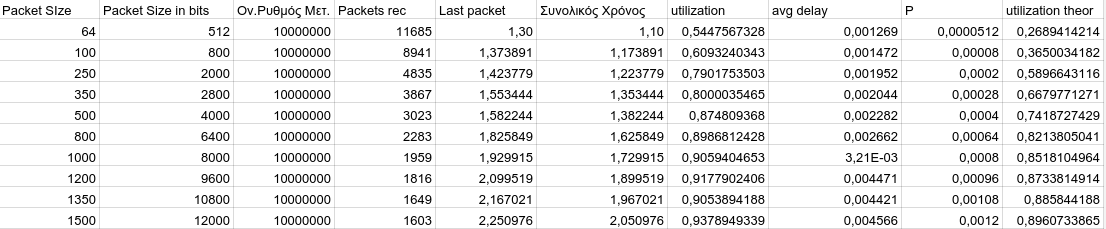
\includegraphics[height=150pt,width=400pt]{spreed1}}
	}
	\qquad \\
	\subfloat[graphs]{{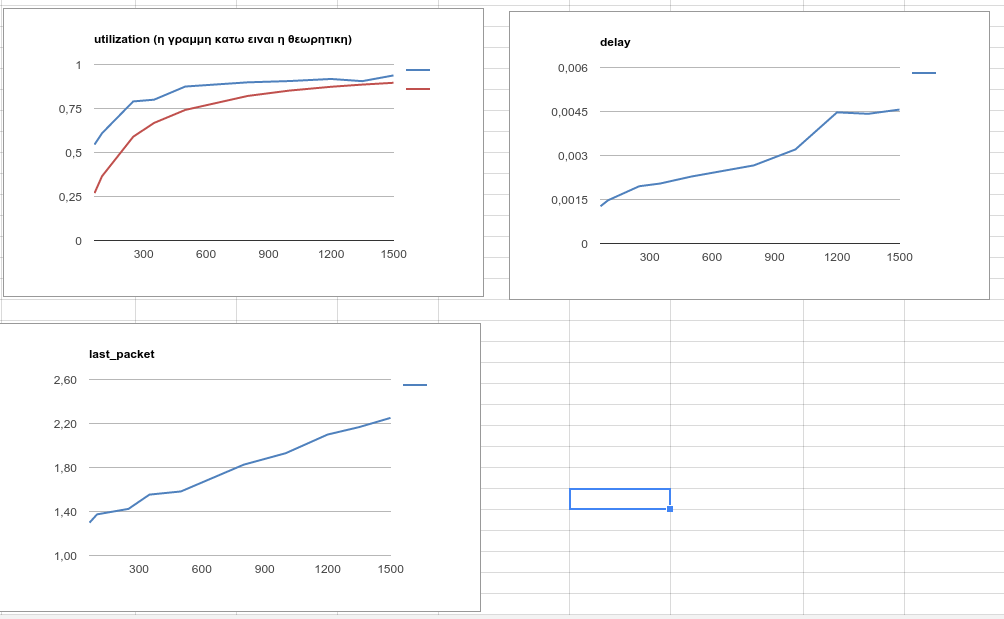
\includegraphics[height=220pt,width=220pt]{graphs1}}}
\end{figure}\\
Από τις γραφικές φαίνεται ότι με μεγαλύτερα πλαίσια έχουμε την χρησιμοποίηση του καναλιού πιο μεγάλη αλλά βέβαια όπως είναι λογικό αυξάνεται η καθυστέρηση κι  ο χρόνος να τελειώσει η αποστολή, εξαιτίας ότι θέλει περισσότερη ώρα να μεταφερθεί ένα μεγαλύτερο πακέτο, έτσι ανάλογα τις ανάγκες μας επιλέγουμε την καταλληλότερη τιμή.Επίσης για την χρησιμοτήτα του καναλιού βλέπουμε ότι κι μαθηματικά ισχύει αυτό από τον τύπο .$\frac{P}{P+2te}\rightarrow \frac{P}{P+c}$ άρα όπως γνωρίζουμε από την ανάλυση για μεγάλα P το κλάσμα προσεγγίζει την μονάδα.
\section*{Problems 4.2}
Εδω χρησιμοποιούμε πάλι το το ίδιο πρόγραμμα κι τα αποτελέσματα ήταν τα εξης
\begin{figure}[ht!]
	\centering
	\subfloat[excel]{{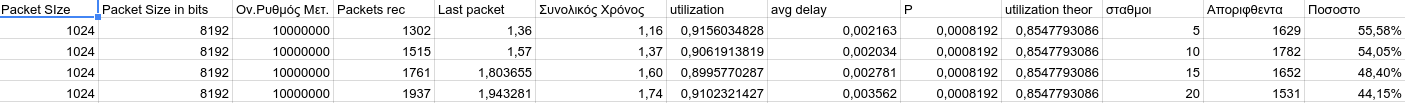
\includegraphics[height=70pt,width=500pt]{s2}}
	}
	\qquad \\
	\subfloat[graphs]{{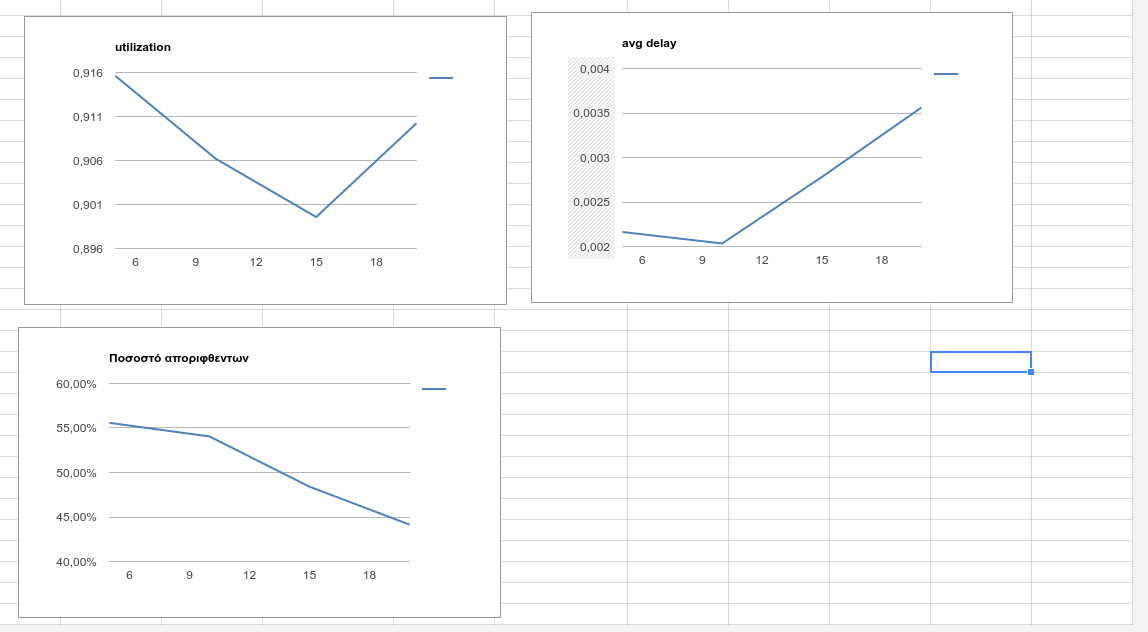
\includegraphics[height=220pt,width=220pt]{graphs2}}}
\end{figure}\\

Παρατηρούμε ότι η χρησιμοποίηση του καναλιού δεν μεταβάλλεται αρκετά , μπορούμε να πούμε ότι παραμένει σχεδόν σταθερή.Η μέση καθυστέρηση αυξάνεται μαζί με την αύξησή των σταθμών γιατί πρέπει να εξυπηρετήσουμε περισσότερους κόμβους.Βλέπουμε πως όσο αυξάνονται οι σταθμοί μειώνεται το ποσοστό των πακέτων που χάνονται αυτό πάλι συμβαίνει γιατί εξαιτίας τον περισσότερον κόμβων διευκολύνεται η μετάδοση κι δεν γεμίζει η γραμμή μας.

Το awk script είναι το ακόλουθο:
\lstinputlisting[language=awk]{lab6.awk}	
\end{document}

